\chapter{Application of remote sensing systems for assessment and prediction of fire risks}
	\label{cha:literature}

	The remote sensing methods are reviewed in this chapter that are used to obtain indirect quantitative and qualitative properties about objects. Passive and active research methods are reviewed. The problems related to the large-scale processing of data for the operative retrieval of results about the object under study are reviewed. Methods for obtaining data from optical and radiometric satellite images are considered.

\section{Application of remote sensing data to the environment}
	Spatial data is one of the fastest growing scientific data, which poses significant computational difficulties for scientists who need to deal with the processing and analysis of large spatial data sets. With the continuous development of sensor technology, the volume of remote sensing images has increased rapidly in recent years and is expected to continue to do so (Yan Ma et al., 2015).
	
	Passive remote sensing data is often used for a variety of environmental challenges:
\begin{itemize}
	\item Wildfire prevention.
	\item Wildfire damage assessment.
	\item Optimization of nitrogen fertilization.
	\item Etc.
\end{itemize}

	For the prevention and detection of forest fire damage, a relative normalized deployment index can be applied (N. V. Rodinov), distinguishing cloud cover and hydrology from the total data array.

	The so-called change detection methodology (CD) can be used to determine forest fire damage. Using the CD methodology, images of different time sections of the same area are usually compared (N. V. Rodinov. Et al., 2016). In order to reduce the images present in the triggers (cloudiness, hydrology), filters are applied to distinguish such triggers using pixel algebra. In this case, the normalized deployment index is calculated for images of different time sections of the same area by making a relative estimate - a relative normalized deployment index. Based on the obtained research results, a data model distinguishing the places where the forest may be affected or most affected is presented.
	
	Currently, more than 100 spectral index variants used for different purposes have been described in different studies using passive remote sensing methods, but only a few of them find wide application in environmental research, monitoring (Vladimir Aleksandrovich Hamedov et al.). In many cases, the described indices do not provide an integrated approach to their complex use in observing a physical phenomenon, which is related to their applications in localized areas using empirical formulas in different ecosystems (Vladimir Aleksandrovis Hamedov et al.). It is for this reason that existing indices used to assess, for example, forest fire risk need to be adjusted for a specific area.
	
	In addition to passive remote sensing, active satellite surveys are increasingly being used, which, for example, make it possible to determine quite accurately:

\begin{itemize}
	\item Water surface contamination by oil products.
	\item Water surface contamination with plastic (plastic).
	\item Fire damage assessment.
	\item Improving fire risk indices.
	\item Etc.
\end{itemize}

	There are a lot of example of successful applying of remote sensing for monitoring and assessment various risk for different environmental purposes:

\begin{example} [Oil detection]
	\label{exa:oil}
	Petroleum products form a film on the surface of the water that is impermeable to sunlight. Without sunlight, the oxidation of bacteria and the multiplication and life of small organisms cease. The death of animal organisms damages the food web. The sea is often polluted by oil products during tanker accidents, but mainly due to sewage from tankers and refineries. Oil products pollute beaches, killing birds and fish.
	
	Large spills of oil products at sea can have significant biological and economic impacts.
	Public and media surveillance is usually intensive after a spill. Remote sensing is playing an increasingly important role in oil monitoring. Active satellite sensors SAR are commonly used to monitor marine oil spills. It is a more effective tool that can penetrate through clouds, rain and snow. The sensor emits microwave radiation that is reflected from the object and the received signal can be determined by the reversible scattering function (Merv Fing et al., 2014).
	
	Active satellite remote sensing has been successfully applied to simulate the 2010 oil spill in Dalian, Japan. In this study, a support vector machine was adapted to monitor oil spills based on high radiometric resolution SAR images (Jianchao Fana et al., 2015).
	
	Under different weather conditions in different places, the reflection and scattering properties of radio waves from the oil differ. On this basis, a vector machine can be constructed that can automatically classify oil spill zones (Jianchao Fana et al., 2015).
	In recent years, water has been increasingly contaminated with plastic products, which need to be monitored and identified to determine the extent of the contamination.
\end{example}

\begin{example}[Plastic detection]
	\label{exa:plastic}
	Plastic pollution in the ocean has been identified as a threat to various coastal areas. Many marine organisms can swallow or become entangled in plastic and this can pose a fatal risk to them. Although high concentrations of floating plastic debris are observed as they travel from inland waters to the open ocean, a detailed analysis of the spatial scale and abundance of waste is lacking and monitoring tools are not well developed to determine the distribution of pollution. Remote-sensing images with medium and high temporal, spectral, and spatial resolutions would be a great additional tool to quantify the distribution of floating marine plastic debris (Shungudzemwoyo P. Garabaa et al., 2017).
	
	Identifying plastics at sea is difficult because there are many different plastics in the marine environment. The size of the plastic can range from microplastics (less than 5 mm) to large plastic parts such as “ghost nets” (lost or discarded fishing nets). In the first case, the plastic material can be toxic through the absorption of contaminants into the plastic, and in the second case, the plastic contaminants can injure animals and endanger seafarers. Plastics can be made from granules used in manufacturing, from certain cosmetic and personal care products, from textile fibers (Lonneke Goddijn-Murphya et al., 2017).
	
	The rays of the sun falling on the surface of the water are partly reflected and the other partially penetrates through the surface. In water, light photons are absorbed and scattered in all directions. Due to the scattering and even distribution of repetitive light rays in all directions, it is possible to identify objects on the water surface. If the water is optically deep (the bottom is invisible), the fraction of light that is scattered and penetrates through the water into the air medium provides information on optically active (e.g., plankton) constituents of the water. Optically active components determine the apparent color of water, and their concentration can be calculated from spectral reflection measurements. In this case, the concentration of plastics can be identified in places where optically active water components cannot be identified (Lonneke Goddijn-Murphya et al., 2017).
	
	Satellites that have sensors that can detect the color of the ocean also provide instruments to identify the plastic, such as Sentinel-3 working in conjunction with Sentinel-3 SLSTR comparing nine bands VIS-SWIR 0.55–12 {$\mu$}m (Lonneke Goddijn-Murphya et al., 2017).
\end{example}

\begin{example} [Nitrogen of plants detection ]
	\label{exa:nitro}
	Optical satellite imagery is by far the most suitable for determining the nitrogen content of plants to reduce the use of fertilizers in crop production.
\end{example}

\begin{example} [Fire risk assessment]
	The estimation of forest fire risk involves the integration of meteorological and other fuel-related variables leading to an index that assesses the different levels of risk. Two indices that are frequently used to estimate the level of fire risk are the Fire Weather Index (FWI) and the Normalized Difference Vegetation Index (NDVI) (ASSESSMENT OF FOREST FIRE RISK IN EUROPEAN MEDITERRANEAN REGION: Comparison of satellite-derived and meteorological indices).
\end{example}	

\section{Open remote sensing data source}

	ESO (European Space Agency) is developing a Sentinel satellite system under the Copernicus program and there is an increasing need for operative analysis in the territory in question to solve various environmental, landscaping and risk management tasks. Such an analysis requires access to constantly updated and high-resolution remote sensing data. Such data are provided by ESO (European Space Agency) under the Copernicus program. The paper examines the application of open Sentinel-1 and Sentinel-2 satellite remote sensing data to address a risk management task, such as fire damage detection.
	
	Sentinel remote sensing data are being developed by ESA under the Copernicus program. This data is free and freely available. In recent years, the need for access to open, free, and frequently updated time-lapse remote sensing data has been growing. Sentinel is divided into 6 groups of satellites, each of which has 2 satellites that can be used to solve various environmental, landscaping and risk management tasks.
	
	One of the most common tasks is risk management. Sentinel data, due to their accuracy and frequent updating in the time section, can be used, for example, to determine fire damage.
	
	ESA has launched two satellites from each Sentinel family into orbit under the ongoing Copernicus program:
	
\begin{itemize}
	\item Sentinel-1 - satellites using active remote sensing sensors. Sentinel-1A launched into orbit in 2014 and Sentinel-1B in 2016.
	\item Sentinel-2 - satellites using multi-spectral high-resolution passive remote sensing sensors. Sentinel-2A was launched into orbit in 2015, and Sentinel-2B in 2017.
	\item Sentinel-3 - multi-functional satellites are used for seabed topography, sea and land surface temperature determination. Used to monitor the environment and climate change. Sentinel-3A was released in 2016 and Sentinel-3B was released in 2018.
	\item Sentinel-4 - geostationary orbit satellites for atmospheric observation.
	\item Sentinel-5 - polar orbit satellites for atmospheric monitoring.
	\item Sentinel-6 is a satellite using an altimeter radar that measures the world's sea level. Used for oceanography and climate research.
\end{itemize}

	Sentinel satellite data is free and publicly available. To receive them, it is necessary to register on the Copernicus Hub website and download them according to the selected search criteria (time, place, etc.). Figure \ref{fig:copernicus_hub} shows a graphical user interface that can be used to download data.

\begin{figure}[H]
	\centering
	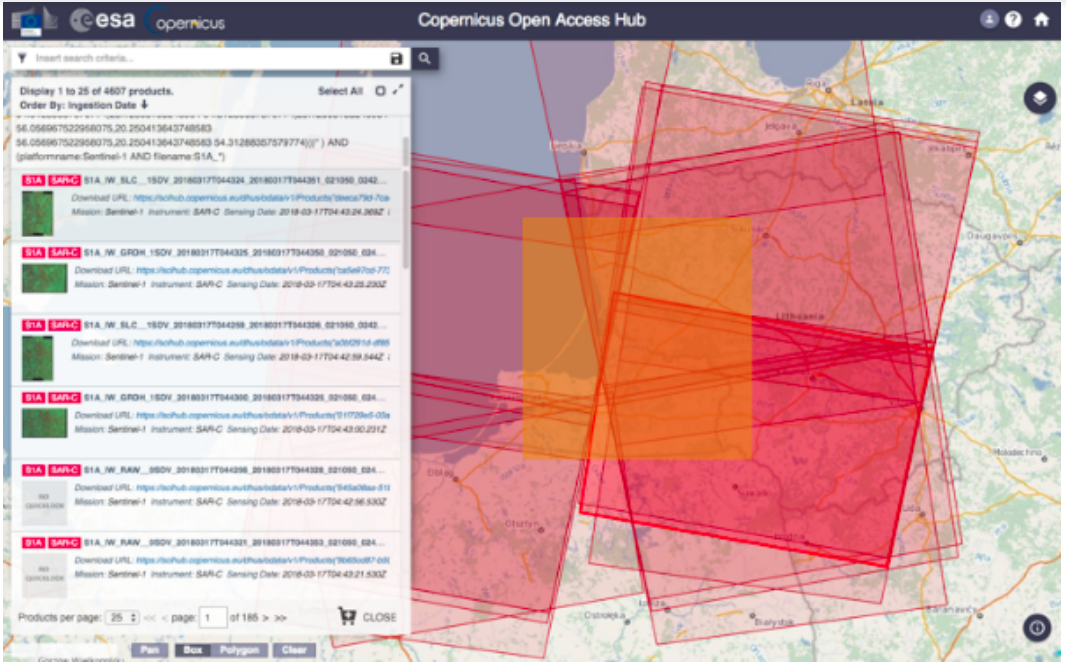
\includegraphics[width=0.8\linewidth]{images/copernicus_hub.png}
	\caption{Sentinel data download via the Copernicus Hub website}
	\label{fig:copernicus_hub}
\end{figure}

	Also the Copernicus Hub programming interface can be used to automate data downloads by specified parameters.
	
	Sentinel data is provided in SAFE (Standard Archive Format for Europe) format. This format stores not only raster information but also textual information that can be used to correct raster data.

\begin{figure}[H]
	\centering
	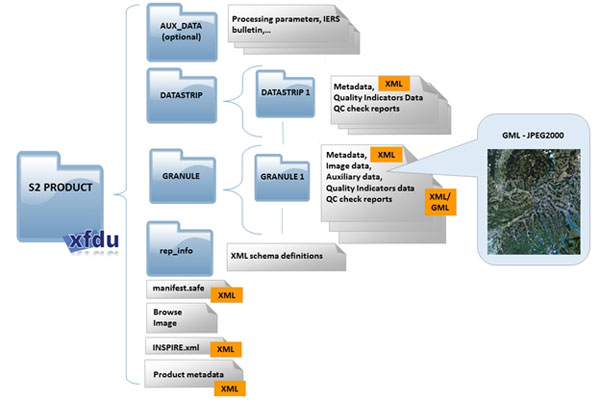
\includegraphics[width=0.8\linewidth]{images/sentinel-2_data_formats.jpg}
	\caption{Example of Sentinel-2 data format}
	\label{fig:sentinel-2_format}
\end{figure}

	The Copernicus program, developed by ESA, provides high-quality and freely available Sentinel satellite data that can be adapted to meet a variety of GIS challenges. One example of such tasks is the identification of fire damage to the forest, the detection of oil spills at sea, the identification of plastic sites at sea. ESA provides all the tools needed for data retrieval (Coperinicus Hub data download portal) and GIS analysis (SNAP software). Sentinel data is high quality, frequently updated, and SNAP free software provides all the tools to perform GIS analysis for both scientific and commercial purposes.

\section{Sentinel passive and active remote sensing systems}
	Remote sensing is the process of obtaining qualitative and quantitative data about a particular object without physical contact.
	Remote sensing systems can be divided into passive and active systems using electromagnetic radiation:
	
	\begin{itemize}
		\item Passive remote sensing systems use an external source of electromagnetic radiation, usually the sun.
		\item Active remote sensing systems have their own light source, which is an electromagnetic wave generator that emits waves from a satellite to the earth's surface. The reflected waves from the earth's surface are captured by a satellite.
	\end{itemize}

	ESA has launched two satellites from each Sentinel family into orbit under the ongoing Copernicus program:
	
	\begin{itemize}
		\item Sentinel-1 - satellites using active remote sensing sensors. Sentinel-1A launched into orbit in 2014 and Sentinel-1B in 2016.
		\item Sentinel-2 - satellites using multi-spectral high-resolution passive remote sensing sensors. Seintinel-2A was launched into orbit in 2015, and Sentinel-2B in 2017.
	\end{itemize}

	Sentinel data is presented in SAFE (Standard Archive Format for Europe) format, which stores not only raster information but also text that can be used to correct raster data, such as cloud cover, so ESA recommends the use of SNAP (Figure 4) open source software for the processing and analysis of their data (\url{http://www.eo4sd-eastern.eu/sites/default/files/publications/snap_workbook_english.pdf}).
	
	Since 2014, radar data (SAR) from the European satellite Sentinel-1A have been freely available, opening up new opportunities for research. The Copernicus portal provides many examples of where they can be applied, ranging from the detection of forest fire damage to the detection of oil spills in water bodies. The main parameters, for example, of Sentinel-1A radar photos (E.A. Baldina et al., 2016):
	
	{\setlength{\extrarowheight}{15pt}%
	\begin{table}[H]
		\begin{center}
			\caption{Sentinel-1A satellite data parameters (E.A. Baldina et al., 2016)}
			\label{tab:sent-char}
			\begin{tabularx}{\textwidth}{|X|X|X|X|}
				\hline
				\textbf{Mode} & \textbf{Coverage area, km} & \textbf{Spatial resolution, m} & \textbf{Polarization\newline(H - horizontal;\newline V - vertical)}\\
				\hline
				Stripmap (SM) & 80 & 5x5 & HH, VV, HH+VV, VV+VH \\
				\hline
				Interferometric Wide Swath (IW) & 250 & 5x20 & HHH, VV, HH+HV, VV+VH \\
				\hline
				Extra-Wide Swath (EW) & 400 & 20x40 & HH, VV, HH+HV, VV+VH \\
				\hline
				Wave (WV) & 20x20 & 5x5 & HH, VV \\
				\hline
			\end{tabularx}
		\end{center}
	\end{table}

	The resolution of the data received by the Sentinel-2A satellite depends on the color wave captured by the sensor and ranges from 10 m to 60 m (tab. \ref{tab:sent-res})).
	
	{\setlength{\extrarowheight}{15pt}%
	\begin{table}[H]
		\begin{center}
			\caption{Sentinel-2A satellite data resolution (Du, Y et al., 2016)}
			\label{tab:sent-res}
			\begin{tabularx}{\textwidth}{|X|X|X|}
				\hline
				\textbf{Physical band} & \textbf{Pixel resolution, m} & \textbf{Wave length, mm}\\
				\hline
				B1 & 60 & 443 \\
				\hline
				B2 & 10 & 490 \\
				\hline
				B3 & 10 & 560 \\
				\hline
				B4 & 10 & 665 \\
				\hline
				B5 & 20 & 705 \\
				\hline
				B6 & 20 & 740 \\
				\hline
				B7 & 20 & 783 \\
				\hline
				B8 & 10 & 842 \\
				\hline
				B8A & 20 & 865 \\
				\hline
				B9 & 60 & 945 \\
				\hline
				B10 & 60 & 1375 \\
				\hline
				B11 & 20 & 1610 \\
				\hline
				B12 & 20 & 2190 \\
				\hline
			\end{tabularx}
		\end{center}
	\end{table}
		
\section{Fire, wildfire and fire risk descriptions}
	Before start moving forward and doing any research we should describe what fire is and what main factors condition it.
	
	Forest fire is a major natural disaster for the European territory. Also known as wildfires, vegetation fires or grass fires, it represents an uncontrolled fire in wild land. It is often caused by human careless or arson and, thus, it is one of the natural disasters more disposable to be prevented by a good preventive scheme.
	
	Forest can be described as an ecosystem characterized by a more or less dense and extensive tree cover, often consisting of stands varying in characteristics such as species composition, structure, age class, and associated processes, and commonly including meadows, streams, fish, and wildlife – note forests include special kinds such as industrial forests, non industrial private forests, plantations, public forests, protection forests, and urban forests, as well as parks and wilderness (Helms 1998).
	
	Forest also can be described as Forest: land with tree crown cover (or equivalent stocking level) of more than 10 \% and area of more than 0.5 ha. The trees should be able to reach a minimum height of 5 m. It may consist either of closed forest formations where trees of various stores and undergrowth cover a high proportion of the ground, or of open forest formations with a continuous vegetation cover in which tree crown cover exceeds 10 \%. Young natural stands and all plantations established for forestry purposes which have yet to reach a crown density of 10 \% or tree height of 5m are included under forest, as are areas normally forming part of the forest area which are temporarily unstocked as a result of human intervention or natural causes but which are expected to revert to forest. The definition of ‘forest’ includes: forest nurseries and seed orchards that constitute an integral part of the forest; forest roads, cleared tracts, firebreaks and other small open areas within the forest; forest in national parks, nature reserves and other protected areas such as those of special environmental, scientific, historical, cultural or spiritual interest; windbreaks and shelter belts of trees with an area of more than 0.5 ha and a width of more than 20 m. Rubber wood plantations and cork oak stands are included. However, the definition of ‘forest’ excludes: land predominantly used for agricultural practices (European Commission 2003).
	
	Fire: rapid burning of combustible material with the evolution of heat and usually accompanied by flame (Encyclopedia Britannica 2005). We can boldly say that forest together with air is a main fuel for a wild fire.
	
	Forest fire is a fire which breaks out and spreads on forest and other wooded land or which breaks out on other land and spreads to forest and other wooded land. The definition of ‘forest fire’ excludes: prescribed or controlled burning, usually with the aim of reducing or eliminating the quantity of accumulated fuel on the ground (European Commission 2003).
	
	A forest fire could occur and evolve assuming different characteristics. Consequently, different types of forest fire have been classified (fig. \ref{fig:fire_types}). The most familiar fire type is the surface fire. It represents the most common propagation regime and consists in rapidly burning fire that sweep quickly over an area, consuming litter and the above ground portions of herbs, shrubs, grasses and lower branches of trees. If conditions are favorable a surface fire may extend to the upper layers of the crown foliage. A fire affecting mainly the crowns of the woody vegetation is called crown fire. Frequently, it leaves most of the steam and the forest floor relatively untouched and is difficult to control since strictly dependent to wind conditions. Moreover, a fire could evolve below the terrain. Referred to as ground fire, it consists principally in largely flame less fire that burn slowly through thick surface accumulation of organic matter, duff and roots and it is very difficult to detect and control. In some particular conditions a ground fire can became a flaming surface fire if not adequately treated (Viegas 2002).

	\begin{figure}[H]
		\centering
		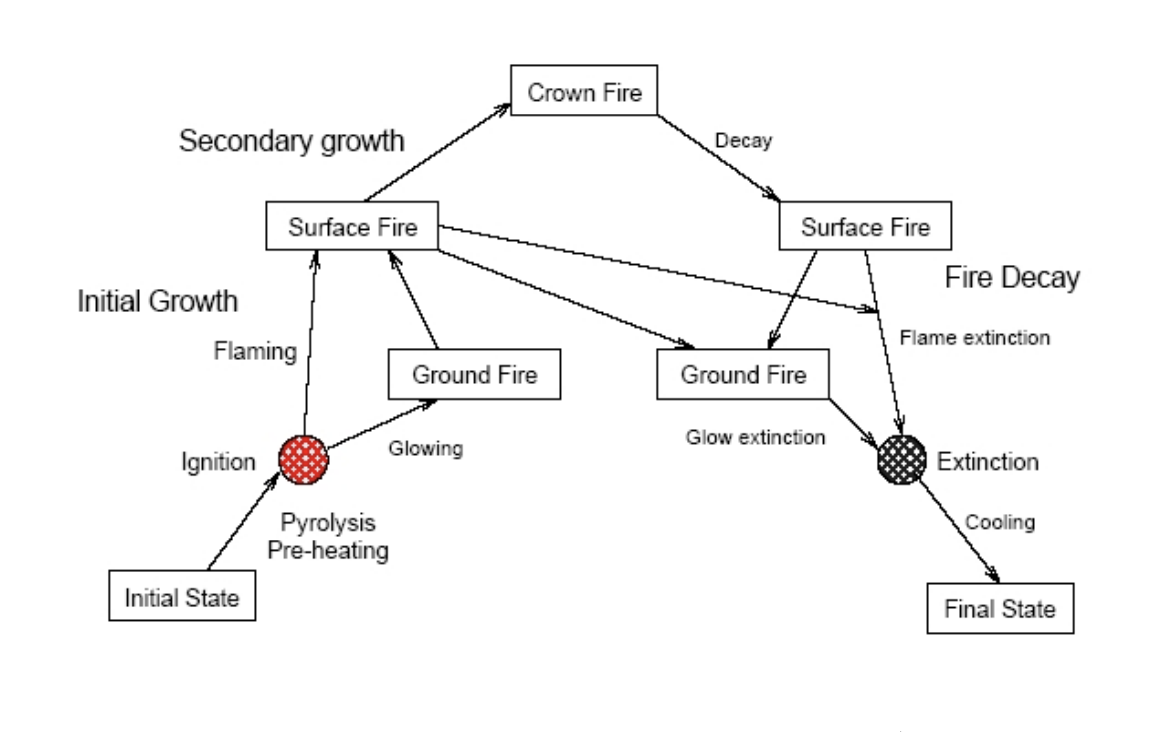
\includegraphics[width=0.9\linewidth]{images/fire_types.png}
		\caption{Fire growth, spread and decay from (Viegas 2002)}
		\label{fig:fire_types}
	\end{figure}

\section{Forest Fire Risk Assessment}
	The evaluation of the effects of a fire a priors is not always possible because the consequences of a forest fire depend by several aspects. Climate conditions, terrain topography, intensity and permanence of the fire are the prevailing elements. Wind condition influences the fire behavior and is really hard to predict. It depends by topography, vegetation and local heating and cooling. Besides, topography may cause dramatic changes in fire behavior as a fire progress over the terrain. In addition, the fire itself may influence the environment and thus the fire behavior; heating from the fire can modify or produce local winds contributing to atmospheric instability and causing cloud development. The effects of fire on soil vary with the proprieties of fuel, fire and soil itself. The consequences are physical, biochemical and biological as well as economic. Fire is able to influence soil temperature, soil structure and the ability of the soil to absorb and store water (Pyne et al. 1996). Forest fires produce gaseous and particle emissions that impact the composition and functioning of the global atmosphere. They are a source of carbon emitted into the atmosphere which influences climate change but are also an irreplaceable sink of carbon. For this reason, the Kyoto protocol, on article 2.ii, suggests the improvement of sustainable forest management practices, afforestation and reforestation.
	
	Fire danger: "the resultant, often expressed as an index, of both constant and variable factors affecting the inception, spread, and difficulty of control of fires and the damage they cause"
	Fire hazard: "a measure of that part of the fire danger contributed by fuels available for burning".
	
	Fire risk: "(1) the chance of fire starting as determined by the presence and activity of causative agents, (2) a causative agent (3) a number related to the potential of firebrands to which a given area will be exposed during the rated day" (FAO 1986).
	
	There are variables changing value almost continuously during the day and variables having a variation noticeable only over a long period of time; week, month or even years. Respectively, these variables were classified as short-term variables and long-term variables. Evapotranspiration, relative humidity, wind and air temperature furnish an example of variables clearly unsteady during the day. Fuel type, fire history, amount of population, topography of the territory, soil type and proximity of roads are variables with a roughly stable behavior in a short period.
	
	
	There are variables changing value almost continuously during the day and variables having a variation noticeable only over a long period of time; week, month or even years. Respectively, these variables were classified as short-term variables and long-term variables.
	
	Evapotranspiration, relative humidity, wind and air temperature furnish an example of variables clearly unsteady during the day. Fuel type, fire history, amount of population, topography of the territory, soil type and proximity of roads are variables with a roughly stable behavior in a short period:
	
	\begin{figure}[H]
		\centering
		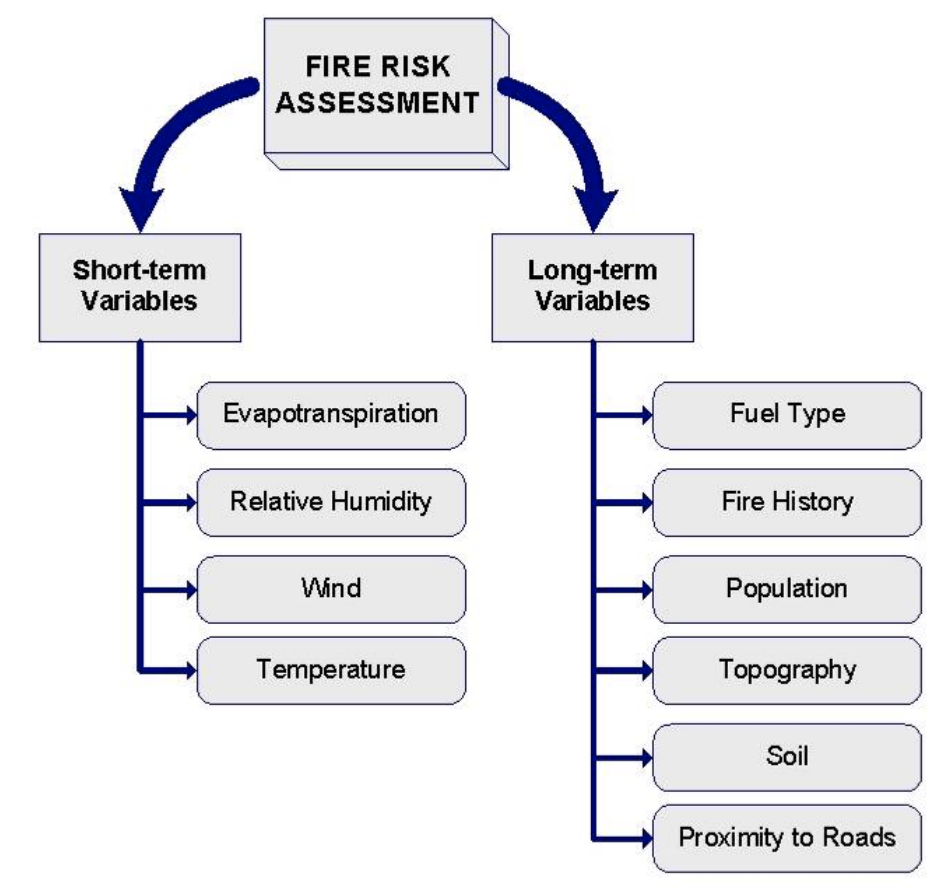
\includegraphics[width=0.8\linewidth]{images/fire_assesment.png}
		\caption{Fire assessments variables}
		\label{fig:copernicus_hub}
	\end{figure}

	In most cases variables on which fire risk depends exist. We can do variables classification into long and short term. Some of them changes continuously and some of them have a variation noticeable only over a long period of time; week, month or even years. We can extract such types of variables:
	
	\begin{itemize}
		\item Meteorological related - fire occurrences and propagation are strongly related to particular meteorological conditions: solar radiation, air temperature, relative humidity, precipitation, wind.
		\item Vegetation related - water retention in plants and in soil is basic to predict moisture content of vegetation; which plays an important role in fire ignition and propagation.
		\item Human behavior related - most of fires causes are directly linked to human behavior. The presence of settlements, agricultural burning, pyromaniacs, barbecues and cigarettes contribute to increase the risk of accidental fires.
	\end{itemize}

\section{Forest fire risk indices}
	An index of risk describes a composite indicator that identifies countries at risk of humanitarian crisis and disaster that would overwhelm national response capacity and it permits to better mange and compare information than using values directly. The values of variables identified as indicators of risk are managed by mathematical expressions. Thus, the result of these expressions is considered in order to extract an index which quantifies the risk throughout a numerical scale.
	
	The indices of wildfire risk can be several. For the sake of simplicity it can be classified in such way:
	
	\begin{itemize}
		\item Long term.
		\item Short term.
	\end{itemize}
	
	\begin{figure}[H]
		\centering
		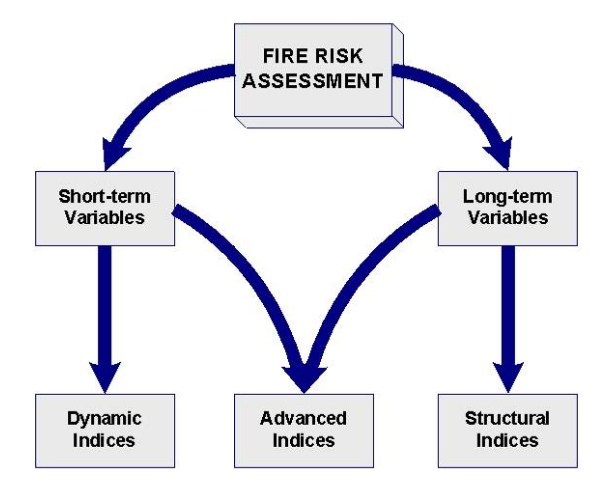
\includegraphics[width=0.8\linewidth]{images/fire_risk_indices.png}
		\caption{Classification of fire risk indices}
		\label{fig:copernicus_hub}
	\end{figure}

\section{Meteorological derived fire risk indices}
	Weather condition have a big impact for risk of wildfire. Depending on solar radiation  or wind speed and direction fire risk can increase dramatically. 
	
	Meteorological factors such as dew point, soil temperature, air temperature, humidity, precipitation and wind speed have
	a major impact on the occurrence of forest fires as these climatic factors change with time and space rapidly (Liu et al., 2015).
	
	The most common meteorological derived fire risk indices used in Europe are:
	
	\begin{itemize}
		\item The Canadian Fire Weather Index (FWI) (Van Wagner 1987).
		\item The Portuguese index (Goncalves and Lourenco 1990).
		\item The Spanish ICONA method - probability of ignition (ICONA 1993).
		\item The Sol Numerical Risk (Drouet and Sol 1993).
	\end{itemize}

	In most cases a correlative data analysis can be used to develop weather index that estimates the risk of forest fires in the interest area (Using correlative data analysis to develop weather index that estimates the risk of forest fires).

\subsection{Canadian Fire Weather Index (FWI)}
	The Canadian Forest Fire Weather Index (FWI) was issued in 1970. It uses four meteorological parameters: noon relative humidity; noon temperature; precipitation during 24 h and the maximum speed of the average wind (Using correlative data analysis to develop weather index that estimates the risk of forest fires).
	
	The FWI System is comprised of six components: three fuel moisture codes (Fine fuel moisture code, Duff Moisture code \& Drought code) and three fire behavior indexes (Initial spread index, Buildup index \& Fire weather index). The mathematical equations of FWI are given below:
	
	\begin{equation}
	B=0.1Rf(d)
	\end{equation}
	
	Where B is the B-scale of FWI readjusted by the factor 0.1, R is the rainfall (mm) and f (d) is the fuel availability ($ft^2$). The final
	S-scale FWI is given bellow:

	\begin{equation}
	ln(s)=2.72[0.434lnB]^{0.647}
	\end{equation}
	
	The Canadian model has been tested and adopted in New Zealand, Fiji, Alaska, Mexico, Chile, Argentina and Europe (Using correlative).
	
	\subsection{The Portuguese index}
		Derived from Nesterov model and based on the assessment of atmospheric conditions in the proximity of the fuel layer:
		
	\begin{equation}
		\begin{aligned}
			x_{k} = y_{k-1} - S\nabla f(y_{k-1})\\
			y_{k} = x_{k} + \dfrac{k-1}{k+2}(x_{k} - x_{x-1})
		\end{aligned}
	\end{equation}

	For any fixed step size $s \le 1/L$, where $L$ is the Lipschitz constant of $\nabla f$, this scheme exhibits the convergence rate (A Differential Equation for Modeling Nesterov’s Accelerated Gradient Method: Theory and Insights).
	
	\subsection{The Spanish ICONA method}
	
	ICONA (Nature Conservation National Institute) adopted one of the classification that was proposed by Rothermel in 1972. That classification distinguishes among 13 fuel models depending on the flame-spreading element. Those models are grouped in four categories:
	
	\begin{itemize}
		\item Pastures.
		\item Scrub.
		\item Leaf litter under tree.
		\item Cutting debris and forestry operations.
	\end{itemize}
	
	\subsection{The Sol Numerical Risk}
	
	The Numerical risk index was developed by Sol in order to improve the prediction of fire occurrence and spread in southern France.
	
	The Numerical risk takes air humidity, soil water reserve and wind speed into account. It requires therefore daily air temperature, dew point temperature, cloud cover, wind speed and potential evapotranspiration (Pereira, A.R., and W.O. Pruitt. 2004. Adaptation of the Thornthwaite scheme for estimating daily reference evapotranspiration. Agricultural Water Management 66: 251-257.) as input variables.
	
	The Numerical risk RN 'is calculated as follows (https://wikifire.wsl.ch/tiki-indexe343.html?page=References):
	
	\begin{equation}
	RN = 25 - \frac{FH WRF WF}{15} + RSF
	\end{equation}
	
	where FH is false relative humidity, WRF the soil water reserve factor, WF the wind factor, and RSF the rate of spread correction factor. FH is calculated as follows:
	
	\begin{equation}
	FH = 100 \frac{e_{s}(T_{dew})}{e_{s}(T_{soil})}
	\end{equation}
	
	where $e_{s}(T_{dew})$ is the saturation vapor pressure at the dew point temperature, and $e_{s}(T_{soil})$ the saturation vapor pressure at the soil (litter) temperature.
	
	The  $e_{s}(T_{soil})$  is derived as follows (temperature at the soil or litter temperature) (Camia \& Bovio 2000):
	
	\begin{equation}
	T_{soil}= \left\{
	\begin{array}{lr}
	 0.874 T -  0.189 U + 11.38, & Cc \leq 2 \\
	 1.36 T - 1.422 Cc - 0.22 T_{dew} + 13.42, & Cc \geq 3
	\end{array} 
	\right.
	\end{equation}
	
	
	where $T$ is air temperature, $U$ wind speed, $Cc$ cloud cover, and $T_{dew}$ dew point temperature.
	
	The soil water reserve factor $WRF$ is calculated as follows:
	
	\begin{equation}
	WRF =  3 + 2 \cdot \tanh(\frac{r - 50}{25})
	\end{equation}
	
	where $\tanh$ is the hyperbolic tangent and r the soil water reserve. 
	
	The wind factor WF is calculated as follows:
	
	\begin{equation}
	WF = 3 + 3 \cdot \tanh(\frac{45 - U}{50})
	\end{equation}
	
	The rate of spread correction factor RSF is determined as follows:
	
	\begin{equation}
	RSF= \left\{
	\begin{array}{lr}
	-3,  & ROS \leq 600 \\
	0,  &  600 < ROS < 1000 \\
	2, & ROS \geq 1000
	\end{array} 
	\right.
	\end{equation}
	
	where ROS, the rate of spread, is calculated as follows:
	
	\begin{equation}
	ROS =  180 \cdot e^{T 1714} \cdot  \tanh(\frac{100 - r}{150} \cdot \{1 + 2 \cdot  (0.8483 + \tanh(\frac{U}{30} - 1.25))\})
	\end{equation}

\section{Vegetation derived fire risk indices}
	Vegetation indices are derived by remote sensing with the aim to attempt to evaluate the vegetation
	stress. They are formed from combinations of several spectral values indicating the amount or vigor of the observed vegetation. The simplest form of vegetation index is a ratio between measurements of reflections in separate portions of the spectrum (Comission).
	
	Indices based on the vegetation stress estimate are called vegetation indices.
	
	A list of the most common indices of vegetation includes: 
	
	\begin{itemize}
		\item The Normalized Difference Vegetation Index (NDVI).
		\item The Soil-Adjusted Vegetation Index (SAVI).
		\item Normalized Difference Water Index.
		\item Relative Greenness Index.
	\end{itemize}

\subsection{The Normalized Difference Vegetation Index (NDVI)}
	The NDVI is the most commonly used index for forest fire risk assessment in which the difference in reflectance is divided by the sum. This compensates for changing illumination conditions, surface slope, aspect, and other extraneous factors and produces a number between -1 and +1. The typical range of actual values is about 0.1 for bare soils to 0.9 for dense vegetation. NDVI is thought to be more sensitive to low levels of vegetative cover (Rouse et al. 1974).
	
	\begin{equation}
	NDVI = \dfrac{\rho_{NIR} - \rho_{red}}{\rho_{NIR} + \rho_{red}}
	\end{equation}
	
	where $\rho_{NIR}$ - near infrared band numerical value and $\rho_{red}$ - red band numerical representation.
	
\subsection{The Soil-Adjusted Vegetation Index (SAVI)}
	This index resembles the NDVI with some added terms to adjust for different brightness of background soil. 
	
	\begin{equation}
	SAVI = \dfrac{\rho_{NIR} - \rho_{red}}{\rho_{NIR} + \rho_{red} + L} \cdot (1 + L)
	\end{equation}
	
	where $\rho_{NIR}$ - near infrared band numerical value and $\rho_{red}$ - red band numerical representation. In principle, the term L can vary from 0 to 1 depending on the amount of visible soil. The constant L is empirically determined to minimize the index sensitivity to soil background reflectance
	variation. However, 0.5 works as a reasonable approximation for L when the amount of soil in the
	scene is unknown and for intermediate vegetation cover ranges. The factor (1+L) set the range of
	SAVI values between -1 and +1, as the range of the NDVI (Huete 1988).

\subsection{Normalized Difference Water Index}
	This index was proposed for remote sensing of vegetation liquid water from space as a complementary
	index for NDVI. The formula Is equivalent to NDVI with the visible channel replaced by a short wave
	infrared reflectance at 1.24 $\mu m$ (Gao 1996).
	
	\begin{equation}
	NDWI = \dfrac{\rho_{NIR} - \rho_{SWIR}}{\rho_{NIR} + \rho_{SWIR} + L} \cdot (1 + L)
	\end{equation}
	
	where $\rho_{NIR}$ - near infrared band numerical value and $\rho_{SWIR}$ - short wave infrared band numerical value.
	
\subsection{Relative Greenness Index}
	It is defined as the relative variation of NDVI, with respect to its maximum and minimum of a long
	period. In this way, the change due to the climatic conditions can be better discriminated, since the absolute value of the NDVI is sometimes more related to the landscape composition instead of seasonal
	dynamism (Goward et al. 1991).
	
	\begin{equation}
	RGI = \dfrac{NDVI_{i} - NDVI_{min}}{NDVI_{max} + NDVI_{min}} \cdot 1000
	\end{equation}

\subsection{Vegetation Moisture Stress}
	For calculation of short term or dynamic components as fire risk indices, the moisture stress could be used.
	The vegetation’s moisture content is another decisive factor for the outbreak and behaviour of a fire.
	The Vegetation Indexes (VIs) are calculated based on the reflectance values in different
	wavelengths, trying to ensure that atmospheric and ground influences are minimal. In this
	paper, the NDII (Normalised Difference Infrared Index) was calculated first, and afterwards, the relative Vegetation Condition Index (VCI) can be calculated:
	
	\begin{equation}
	VCI_{i}=[(NDII_{i} - NDII_{min})/(NDII_{max} - NDII_{min})] \cdot 100
	\end{equation}
	
	where $VCI_{i}$ is the Vegetation Condition Index for each date; $NDII_{i}$ is the index for dryness on the date in question; $NDII_{min}$ is the index of minimum dryness and $NDII_{min}$ is the index of maximum dryness for given oeriod.

\section{Processing of remote sensing data using distribution systems}
	At present, remote sensing and GIS methods used to process remote sensing data are a powerful tool for studying, predicting and non-invasive monitoring of environmental change.
	The term "remote sensing" is widely used to describe a method of collecting information about the Earth's surface without contact with it. The electromagnetic energy reflected or emitted during remote sensing is recorded by a sensor in the form of an image. These images are then processed and analyzed to obtain meaningful information about the objects and phenomena depicted. Remote sensing is a multi-stage process involving several components and the interactions between them. Remote sensing requires an energy source. Currently, two types of remote sensing sensors are used - passive and active. In terms of passive remote sensing, solar energy reaches the Earth, interacting with the atmosphere and objects on the Earth’s surface. The reflected part of this energy is received by the sensor, encoded by electrical signals and transmitted to the ground station. To become valuable, this data needs to be prepared, corrected, and improved. Further processing involves intensive decryption and analysis, which allows the data to be turned into meaningful information. Increasingly, remote sensing data is processed using so-called “learning systems,” where neural network methodologies create a system that can process large amounts of data automatically, without human intervention (P. Scheunders D. et al., 2017; Atharva Sharma et al., 2017).
	
	With active remote sensing, the sensor sends a signal (in the case of a satellite, generated radio waves) that is reflected from the earth's surface, interacting with objects on it, and returns to the sensor's recorder.
	
	Currently, passive remote sensing (using optical satellite imagery) is commonly used in conjunction with GIS to:

	\begin{itemize}
		\item Manage, monitor the consequences of natural disasters.
		\item Anticipate the possible consequences of future natural disasters.
	\end{itemize}
	
	Many tools and methods have been developed, in particular:
	
	\begin{itemize}
		\item Land management.
		\item Management and analysis of cultural and natural heritage areas.
		\item In geology.
		\item In hydrology.
		\item In navigation.
		\item In geodesy and cartography.
	\end{itemize}

	Many methodologies have been developed that are applicable to optical satellite imagery, but there are several problems with the application of passive remote sensing techniques:
	
	\begin{itemize}
		\item There is no possibility to perform tests at any time of the day.
		\item Weather conditions (cloudiness) limit the use of optical photographs.
		\item Studies based on the optical properties of light rays (reflection, absorption, deflection) do not. \item Always show accurate results.
	\end{itemize}

	Some of these problems can be solved by using active remote sensing - radiometric satellite imagery:
	
	\begin{itemize}
		\item Tests can be performed at any time of the day.
		\item Weather conditions do not restrict the use of satellite imagery.
		\item Radiometric photographs provide more accurate results.
	\end{itemize}

	The main disadvantage of using active remote sensing is that most methods and algorithms for processing radiometric images require larger computations, and the algorithms themselves are complex.
	In order to process remote sensing data quickly and efficiently, it is necessary to apply distributed calculations:
	
	\begin{itemize}
		\item Cluster of computers.
		\item Cloud solutions;
	\end{itemize}
	
	Many GIS software packages do not yet use the full capacity of computers to process remote sensing data. Modern processors are made up of cores that can process data in parallel, thus speeding up the processing of remote sensing data. The paper examines methods that allow the use of distributed computations, as well as a methodology to accelerate their processing independently of remote sensing data processing algorithms to provide real-time data that could be used to monitor and analyze environmental parameters (Michael McCool Arch D. et al. 2012).
	
	By accelerating the processing of remote sensing data, active satellite imagery can be adapted to detect the following phenomena:
	
	\begin{itemize}
		\item Determination of water surface contamination by petroleum products using active remote sensing (Syntetic Aperture Radar).
		\item Determination of water surface contamination with plastic (plastic products) using active remote sensing.
		\item To monitor plastic contamination of the earth's surface using active remote sensing.
		\item To assess the damage caused by a forest fire and to determine the direction of fire expansion.
		\item Determination of nitrogen content in plants in order to reduce the use of fertilizers in crop production.
		\item Determination of air pollution using active remote sensing.
	\end{itemize}
	
	Remote sensing of satellite systems can provide ecologically sound long-term data sets suitable for analyzing changes in the ecosystem in a given area, in terms of structure, time and space, using appropriate risk assessment criteria. It is often complex and unclear how to select and effectively use remotely obtained data that could be used for environmental parameters and risk assessment (Jining Yana et al., 2017).
	
	Data obtained by remote sensing are often difficult to adapt due to the complexity of their processing. Often, satellite survey data cannot be processed fully automatically and their results must be interpreted with caution. It is for these reasons that it is often necessary to adapt processing and outcome evaluation methodologies to the area in which the research is conducted (Atharva Sharma et al., 2017).
	Automatic interpretation of remote sensing images is a very complex problem and is fast becoming a necessity for many areas such as disaster management, forest mapping, urban planning, and more. Indeed, images with ever-increasing spatial resolution are becoming such that their adaptation becomes difficult without any computer aid (Hui He et al., 2016).
	
	Sometimes it is not possible to process existing data by adapting computer programs because they do not use the full capacity of the computer. Despite the fact that computer hardware is naturally parallel, computer architects decided 40 years ago to accept serial programming abstraction for programmers (fig. \ref{fig:seq_exec}).
	
	\begin{figure}[H]
		\centering
		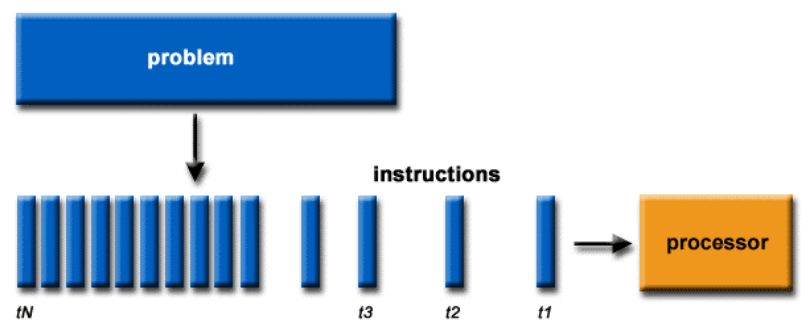
\includegraphics[width=0.9\linewidth]{images/seq_exec.png}
		\caption{Serial execution of instructions on a simple processor}
		\label{fig:seq_exec}
	\end{figure}

	Decades of computer architecture have been designed to maintain the illusion of series execution. In modern processors, much effort is put into translating serial programs into parallel form so that they can run efficiently using parallel hardware inside the processor. Unfortunately, despite the increase in the number of transistors provided for in Moore's Law (which states that the number of transistors that can be integrated into a chip doubles every two years), the need for parallelism is now so great that the illusion of serial computing cannot be maintained (Michael McCool Arch D. et al., 2012).
	
	Serial execution of computer operations is not optimized and GIS problem solving can be accelerated by applying algorithms that specify how operations should be performed in parallel.
	
	Parallel computations and data processing are several computational resources at the same time when those resources are automatically allocated to solve the problem:
	
	\begin{itemize}
		\item The problem is broken down into several separate parts that can be solved at the same time.
		\item Each part is divided into separate series of instructions.
		\item Each instruction in the series is executed simultaneously using all computer resources in parallel.
	\end{itemize}

	\begin{figure}[H]
		\centering
		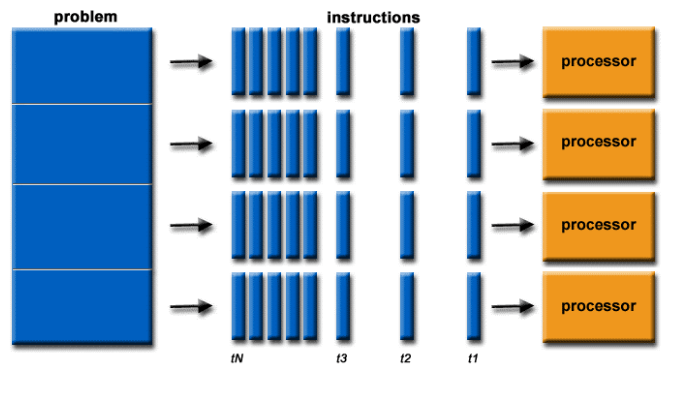
\includegraphics[width=0.9\linewidth]{images/par_exec.png}
		\caption{Parallel execution of instructions on a simple processor}
		\label{fig:par_exec}
	\end{figure}
	